\documentclass[11pt,a4paper]{article}

\usepackage{url}
\usepackage{graphicx}
\usepackage{amsfonts}
\usepackage{amssymb}
\usepackage{amsmath}
\usepackage{amsfonts}
\usepackage{amssymb}
\usepackage{amsmath}
\usepackage{multirow}
\usepackage{listings}
\usepackage{fullpage}
\usepackage{fancyhdr,a4wide}
\usepackage{makeidx}
\usepackage{placeins}
\usepackage[procnames,noindent]{lgrind}

\lstset{ %
language=VHDL,                % choose the language of the code
basicstyle=\footnotesize,       % the size of the fonts that are used for the code
showstringspaces=false,         % underline spaces within strings
%numbers=left,                   % where to put the line-numbers
%numberstyle=\footnotesize,      % the size of the fonts that are used for the line-numbers
%stepnumber=1,                   % the step between two line-numbers. If it's 1 each line will be numbered
%numbersep=5pt,                  % how far the line-numbers are from the code
%backgroundcolor=\color{white},  % choose the background color. You must add \usepackage{color}
showspaces=false,               % show spaces within strings adding particular underscores
showtabs=false,                 % show tabs within strings adding particular underscores
escapeinside={\%*}{*)}          % if you want to add a comment within your code
}

\begin{document}	

\begin{titlepage}

\thispagestyle{fancy}
\lhead{}
\chead{
\large{\textit{
Informatics and Mathematical Modelling\\
Technical University of Denmark}}}
\rhead{}
\rule{0pt}{50pt}
\vspace{3cm}

\begin{center}

 	\huge{\textbf{02207 : Advanced Digital Design Techniques}}\\
 	\vspace{1cm}
 	\huge{Lab 1: Exercise on Synthesis}\\
 	\vspace{1cm}
 	\huge{Group \textit{dt07}}\\	
\end{center}

\vspace{4cm}

\begin{flushright}
	\LARGE{Markku Eerola (s053739)}\\
	\vspace{0.3cm}
	\LARGE{Rajesh Bachani (s061332)}\\
	\vspace{0.3cm}
	\LARGE{Josep Renard (s071158)}\\
\end{flushright}
\cfoot{\today}
\end{titlepage}

%\begin{abstract}
%\centering
%Abstract to be created.
%\end{abstract}

%-----------------------------------------------------------
\newpage 
\tableofcontents

\newpage 
\section{Purpose of the Exercise}

The goal of the exercise was to get familiar with the process of synthesis of digital circuits, using special tools for synthesis such as Design Vision. A register-level netlist containing a 24-bit adder is synthesized in the exercise, for different values of the clock time period. The reports concerning the timing constraints, area, power consumption etc. which are generated by the tool are documented in the report.

\section{Behavioral Description for 24-bit Adder}

\subsection{VHDL code for the 24-bit Adder}
% Describe something about the adder %
The VHDL code for a simple 24-bit adder is provided below.\\ 

\lstinputlisting[frame=trbl]{../source/NBitAdder.vhdl}

\subsection{Simulation with Modelsim}
The behavior of this adder is verified in Modelsim. Following is a testbench for the adder, and also a screenshot for the waveform from the values provided by the testbench.

\lstinputlisting[frame=trbl]{../source/tbnadder.vhdl}

\begin{figure}[htp]
\centering
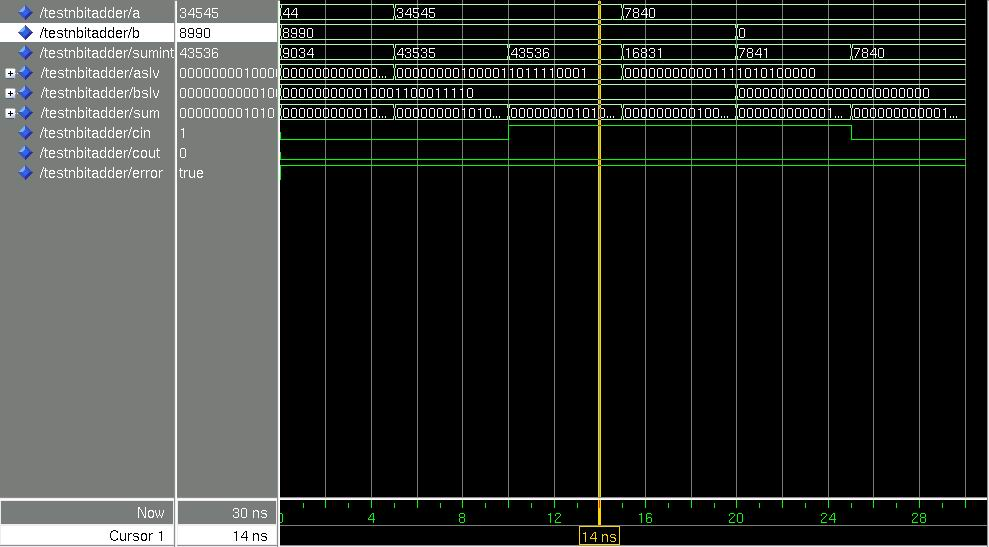
\includegraphics[width = 6in]{../source/wave.jpg}
\end{figure}

As we can see, the values of a, b and cin at the point of the yellow line are 34545, 8990 and 1. The resulting sum is shown as 43536, which is correct. Even for the other values in the testbench, we can verify the adder is working fine.

\section{Behavioral Description for 24-bit Register}

The VHDL code for a 24-bit register is provided below.\\ 

\lstinputlisting[frame=trbl]{../source/reg.vhdl}

\section{Top-Level Netlist from 24-bit Adder and 24-bit Register}
\label{sec:netlist}

The VHDL code for the top-level netlist described in the exercise sheet, is provided below.\\ 
\lstinputlisting[frame=trbl]{../source/addernetlist.vhdl}

\section{Synthesis Results}

The synthesis of the top-level netlist described in section \ref{sec:netlist} is done using Design Vision by Synopsys. We have synthesized the netlist for three different sets of clock time periods, which are 0.5, 1.0 and 2.0 ns. For each of these time periods, we have synthesized the netlist with and without constraints for low power. In the end, we have commented on the results obtained from the data gathered.

The power constraints for low power are 1 uW and 1 pW for maximum dynamic power and maximum leakage power respectively. This is done by using the following two commands (as is also shown in the exercise sheet):\\

\begin{lstlisting}[frame=trbl]{}
set_max_dynamic_power 1
set_max_leakage_power 1
\end{lstlisting}
\vspace{0.5cm}
For the synthesis in which no constraints are put on power, the values are kept at 10 mW and 30 uW for maximum dynamic power and maximum leakage power respectively.\\

\begin{lstlisting}[frame=trbl]{}
set_max_dynamic_power 10 mW
set_max_leakage_power 30 uW
\end{lstlisting}
\vspace{0.5cm}

In the following subsections, we give the results and comments of the synthesis for both the above mentioned power constraints. In the end of the section, we give comments and justification for the change in area and power with respect to the clock period of synthesis.

\newpage
\subsection{Clock Time Period = 0.5 ns}
\begin{table}[htbp]
\begin{center}
\begin{tabular}{|l|l|l|}
\hline
\textbf{Parameters}	& \textbf{Values}		& \textbf{Comment}\\ \hline
Dynamic Power				&	5.91 mW				& MET\\ \hline
Leakage Power 			&	11.04 uW			& MET\\ \hline
Library Setup Time  & 0.08 ns				& - \\ \hline
Data Arrival Time		& 0.43 ns				& - \\ \hline
SLACK								& -0.01 ns			& VIOLATED \\ \hline
Combinational Area	& 2700 um^2			& - \\ \hline
Non-Combinational Area	& 1343 um^2	& - \\ \hline
SVT cells						& 403						& - \\ \hline
HVT cells						& 0							& - \\ \hline
\end{tabular}
\end{center}
\caption{}
\label{tab:syn0.5.1}
\end{table}

Synthesis for low power:

\begin{table}[htbp]
\begin{center}
\begin{tabular}{|l|l|l|}
\hline
\textbf{Parameters}	& \textbf{Values}		& \textbf{Comment}\\ \hline
Dynamic Power				&	5.29 mW				& VIOLATED\\ \hline
Leakage Power 			&	9.22 uW				& VIOLATED\\ \hline
Library Setup Time  & 0.08 ns				& - \\ \hline
Data Arrival Time		& 0.44 ns				& - \\ \hline
SLACK								& -0.02 ns			& VIOLATED \\ \hline
Combinational Area	& 2345 um^2			& - \\ \hline
Non-Combinational Area	& 1343 um^2	& - \\ \hline
SVT cells						& 377						& - \\ \hline
HVT cells						& 0							& - \\ \hline
\end{tabular}
\end{center}
\caption{}
\label{tab:syn0.5.2}
\end{table}

\newpage
\subsection{Clock Time Period = 1.0 ns}
\begin{table}[htbp]
\begin{center}
\begin{tabular}{|l|l|l|}
\hline
\textbf{Parameters}	& \textbf{Values}		& \textbf{Comment}\\ \hline
Dynamic Power				&	2.76 mW				& MET\\ \hline
Leakage Power 			&	11.25 uW			& MET\\ \hline
Library Setup Time  & 0.08 ns				& - \\ \hline
Data Arrival Time		& 0.89 ns				& - \\ \hline
SLACK								& 0.02 ns				& MET\\ \hline
Combinational Area	& 2335 um^2			& - \\ \hline
Non-Combinational Area	& 1343 um^2	& - \\ \hline
SVT cells						& 276						& - \\ \hline
HVT cells						& 0							& - \\ \hline
\end{tabular}
\end{center}
\caption{}
\label{tab:syn1.0.1}
\end{table}

Synthesis for low power:

\begin{table}[htbp]
\begin{center}
\begin{tabular}{|l|l|l|}
\hline
\textbf{Parameters}	& \textbf{Values}		& \textbf{Comment}\\ \hline
Dynamic Power				&	1.71 mW				& VIOLATED\\ \hline
Leakage Power 			&	2.98 uW				& VIOLATED\\ \hline
Library Setup Time  & 0.09 ns				& - \\ \hline
Data Arrival Time		& 0.90 ns				& - \\ \hline
SLACK								& 0.00 ns				& MET\\ \hline
Combinational Area	& 1089 um^2			& - \\ \hline
Non-Combinational Area	& 1343 um^2	& - \\ \hline
SVT cells						& 205						& - \\ \hline
HVT cells						& 0							& - \\ \hline
\end{tabular}
\end{center}
\caption{}
\label{tab:syn1.0.2}
\end{table}

\newpage
\subsection{Clock Time Period = 2.0 ns}
\begin{table}[htbp]
\begin{center}
\begin{tabular}{|l|l|l|}
\hline
\textbf{Parameters}	& \textbf{Values}		& \textbf{Comment}\\ \hline
Dynamic Power				&	0.896 mW			& MET\\ \hline
Leakage Power 			&	3.51 uW				& MET \\ \hline
Library Setup Time  & 0.09 ns				& - \\ \hline
Data Arrival Time		& 1.87 ns				& - \\ \hline
SLACK								& 0.05 ns				& MET \\ \hline
Combinational Area	& 631 um^2			& - \\ \hline
Non-Combinational Area	& 1343 um^2	& - \\ \hline
SVT cells						& 97						& - \\ \hline
HVT cells						& 0							& - \\ \hline
\end{tabular}
\end{center}
\caption{}
\label{tab:syn2.0.1}
\end{table}

Synthesis for low power:

\begin{table}[htbp]
\begin{center}
\begin{tabular}{|l|l|l|}
\hline
\textbf{Parameters}	& \textbf{Values}		& \textbf{Comment}\\ \hline
Dynamic Power				&	0.88 mW				& MET\\ \hline
Leakage Power 			&	3.17 uW				& VIOLATED\\ \hline
Library Setup Time  & 0.09 ns				& - \\ \hline
Data Arrival Time		& 1.91 ns				& - \\ \hline
SLACK								& 0.00 ns			& MET\\ \hline
Combinational Area	& 614 um^2			& - \\ \hline
Non-Combinational Area	& 1343 um^2	& - \\ \hline
SVT cells						& 97						& - \\ \hline
HVT cells						& 0							& - \\ \hline
\end{tabular}
\end{center}
\caption{}
\label{tab:syn2.0.2}
\end{table}

\FloatBarrier
\section{Discussion}


\end{document}